\documentclass[12pt]{book}
% !TEX root = hazy2.tex
%\includeonly{limits}
%\includeonly{coninter}
%\includeonly{lineatomparam}
%\includeonly{linedetl}
%\includeonly{codestruc}
%\includeonly{CloudyStandaloneProgram}
%\includeonly{sub}
%\includeonly{output}
%\includeonly{observed}
%\includeonly{lines}
%\includeonly{problems}
%\includeonly{odetail}
%\includeonly{sources}
%\includeonly{glossary}
%\includeonly{conversion}
%\includeonly{TestSuite}
%\includeonly{refer}

\usepackage{graphicx,rotate,url,mathptmx,lscape,times,framed,color}

% include natbib for bibtex, options are
% round use (2008) instead of [2008] for year
\usepackage[round]{natbib}

% cross references across documents
\usepackage{xr}

%\begin{comment}
%This is my comment.
%Note that it can span multiple lines.
%This is very useful.
%\end{comment}
\usepackage{verbatim} 

% allow hyperlinks
\usepackage{hyperref}
\hypersetup{
    bookmarks=true,         % show bookmarks bar?
    unicode=false,          % non-Latin characters in Acrobat�s bookmarks
    pdftoolbar=true,        % show Acrobat�s toolbar?
    pdfmenubar=true,        % show Acrobat�s menu?
    pdffitwindow=true,      % page fit to window when opened
    pdftitle={My title},    % title
    pdfauthor={Author},     % author
    pdfsubject={Subject},   % subject of the document
    pdfnewwindow=true,      % links in new window
    pdfkeywords={keywords}, % list of keywords
    colorlinks=true,        % false: boxed links; true: colored links
    linkcolor=blue,         % color of internal links, def red
    citecolor=blue,         % color of links to bibliography, def green
    filecolor=blue,         % color of file links, def magenta
    urlcolor=blue           % color of external links, def cyan
}

% geometry package controls page layout
\usepackage[letterpaper,
left=2.5cm,right=2.5cm,
top=2.5cm,bottom=2.5cm]{geometry}
\oddsidemargin=+0.7cm
\evensidemargin=-0.7cm
\pagestyle{headings}

% journal name macros used by ADS
\usepackage{../common/aas_macros}

% Include list of figures and references in contents lists
\usepackage[nottoc]{tocbibind}

% makes it easy to include all or part of a PDF document 
% inside a LaTeX document
\usepackage{pdfpages}

% allow external files to be included verbatim
\usepackage{moreverb}
% set the default tabsize
\def\verbatimtabsize{4\relax}

% following are to pick up .aux files for cross references
% with package xr to other volumes of Hazy
% hazy 1
\externaldocument[Hazy1-]{../hazy1/intro}
\externaldocument[Hazy1-]{../hazy1/define}
\externaldocument[Hazy1-]{../hazy1/cmdintro}
\externaldocument[Hazy1-]{../hazy1/cont-def}
\externaldocument[Hazy1-]{../hazy1/cont-lum}
\externaldocument[Hazy1-]{../hazy1/cont-shp}
\externaldocument[Hazy1-]{../hazy1/compos}
\externaldocument[Hazy1-]{../hazy1/density}
\externaldocument[Hazy1-]{../hazy1/geometry}
\externaldocument[Hazy1-]{../hazy1/optdepth}
\externaldocument[Hazy1-]{../hazy1/therm}
\externaldocument[Hazy1-]{../hazy1/dynamics-time}
\externaldocument[Hazy1-]{../hazy1/stopping}
\externaldocument[Hazy1-]{../hazy1/conout}
\externaldocument[Hazy1-]{../hazy1/optimize}
\externaldocument[Hazy1-]{../hazy1/grid}
\externaldocument[Hazy1-]{../hazy1/miscell}
\externaldocument[Hazy1-]{../hazy1/latex_style}

% hazy2
\externaldocument[Hazy2-]{../hazy2/limits}
\externaldocument[Hazy2-]{../hazy2/coninter}
\externaldocument[Hazy2-]{../hazy2/lineatomparam}
\externaldocument[Hazy2-]{../hazy2/linedetl}
\externaldocument[Hazy2-]{../hazy2/CloudyStandaloneProgram}
\externaldocument[Hazy2-]{../hazy2/sub}
\externaldocument[Hazy2-]{../hazy2/output}
\externaldocument[Hazy2-]{../hazy2/observed}
\externaldocument[Hazy2-]{../hazy2/lines}
\externaldocument[Hazy2-]{../hazy2/problems}
\externaldocument[Hazy2-]{../hazy2/odetail}
\externaldocument[Hazy2-]{../hazy2/sources}
\externaldocument[Hazy2-]{../hazy2/glossary}
\externaldocument[Hazy2-]{../hazy2/conversion}
\externaldocument[Hazy2-]{../hazy2/TestSuite}

% hazy 3
\externaldocument[Hazy3-]{../hazy3/isoseq}
\externaldocument[Hazy3-]{../hazy3/hydroiso}
\externaldocument[Hazy3-]{../hazy3/helikeiso}
\externaldocument[Hazy3-]{../hazy3/molecules}
\externaldocument[Hazy3-]{../hazy3/dheavy}
\externaldocument[Hazy3-]{../hazy3/dtherm}
\externaldocument[Hazy3-]{../hazy3/dgrain}
\externaldocument[Hazy3-]{../hazy3/dother}

% set paragraph styles
\raggedright
\setlength{\parindent}{4mm}
% background color for shaded boxes
\definecolor{shadecolor}{gray}{0.9}

% Customize contents details from book.cls
\makeatletter

\renewcommand*\l@section{\@dottedtocline{1}{1.5em}{3.1em}}
\renewcommand*\l@subsection{\@dottedtocline{2}{4.6em}{4.1em}}
\renewcommand*\l@subsubsection{\@dottedtocline{3}{8.7em}{5.1em}}
\renewcommand*\l@paragraph{\@dottedtocline{4}{10em}{6em}}
\renewcommand*\l@subparagraph{\@dottedtocline{5}{12em}{7em}}
\renewcommand*\l@figure{\@dottedtocline{1}{1.5em}{3.3em}}

% extract name of target of reference (e.g. chapter titles)
\long\def\@thirdoffive#1#2#3#4#5{#3}%
\def\refname#1{\expandafter\@setref\csname r@#1\endcsname\@thirdoffive{#1}}

% create ruler underneath page header
\advance\headheight1.2pt
\def\@oddhead{\vbox{\parindent=0pt%
\setbox0=\hbox to\textwidth{{\slshape\rightmark}\hfil\thepage}%
\dimen0=4.5pt \advance\dimen0 by-\dp0 \box0\kern\dimen0\hrule}}
\def\@evenhead{\vbox{\parindent=0pt%
\setbox0=\hbox to\textwidth{\thepage\hfil\slshape\leftmark}%
\dimen0=4.5pt \advance\dimen0 by-\dp0 \box0\kern\dimen0\hrule}}

% modify font size for verbatim environment
\newcommand{\setverbatimfontsize}[1]{\renewcommand*\verbatim@font{#1\ttfamily}}
\renewcommand*\verbatim@font{\footnotesize\ttfamily}

% Change title of bibliography
\renewcommand\bibname{REFERENCES}
\renewcommand\contentsname{CONTENTS}
\renewcommand\listfigurename{LIST OF FIGURES}
\renewcommand\listtablename{LIST OF TABLES}
% tweak bibliograpy environment to be more like old Hazy
\def\thebibliography#1{%
\bibsection
\@mkboth{\MakeUppercase\bibname}{\MakeUppercase\bibname}%
\list{}{\setlength\labelwidth{2.5em}\leftmargin\labelwidth
\setlength\parsep{0pt}\setlength\itemsep{0.7mm plus1pt}
\setlength{\itemindent}{-\leftmargin}
\small}
\def\newblock{\hskip .11em plus .33em minus -.07em}
\sloppy
\sfcode`\.=1000\relax}
\def\endthebibliography{\endlist}

\makeatother
% End of contents customization

\input{../common/macros}
\input{../variables}

\externaldocument[Hazy1-]{../hazy1/hazy1}
\externaldocument[Hazy1-]{../hazy1/conout}

\begin{document}
\frontmatter

%%%%%%%%%%%%%%%%%%%%%%%%%%%%%%%%%%%%%%%%%%%%%%%
%  title page
\begin{titlepage}
\begin{center}

\Huge
Hazy\\
\Large
\emph{a brief introduction to \Cloudy\ C\VERSION}\\
\LARGE
2. Results, computational environment,\\
and test suite

\begin{figure}
\begin{center}
\includegraphics[clip=on,width=0.8\columnwidth,keepaspectratio]{coll_t7}
\end{center}
\end{figure}

\vspace{15 mm }
\LARGE
\emph{Cloudy \& Associates} \\
\Large
\href{http://www.nublado.org}{www.nublado.org} \\
\normalsize
\today
\end{center}
\end{titlepage}

%%%%%%%%%%%%%%%%%%%%%%%%%%%%%%%%%%%%%%%%%%%%%%%
% page with one figure and boilerplate text
\clearpage
\input{../frontis_common}
\vspace{5mm}
\noindent
{\small
{\em Cover image:} The spectrum emitted by a cloud with solar abundances,
a temperature of 10$^7$~K, a density of 10$^{10} \pcc$, and a column density
of 10$^{15} \pscm$.  This shows recent improvements in the X-ray spectrum
and was done with the test case \cdFilename{coll\_t7.in} located in
\cdFilename{tsuite/auto}.  The command
\cdCommand{set continuum resolution 0.1} was added to
increase the continuum resolution by a factor of ten.
}
\clearpage

%%%%%%%%%%%%%%%%%%%%%%%%%%%%%%%%%%%%%%%%%%%%%%%
% table of contents page - only include top two levels
\setcounter{tocdepth}{2}
\tableofcontents
\listoffigures
\listoftables

\clearpage
\mainmatter
\include{output}       %proof 1
\chapter{OBSERVED QUANTITIES}
% !TEX root = hazy2.tex
\label{sec:ObservedQuantities}

\section{Overview}

This section describes how to convert the quantities actually used or
predicted by \Cloudy\ into commonly observed ones.

\section{Intensities of various continua}

\subsection{Incident radiation field}

The incident radiation field is the light striking the cloud.
The
main printout printout gives the intensity of the
incident radiation field with
the label ``Inci''.
The total continuum [units erg s$^{-1}$ or erg cm$^{-2}$~s$^{-1}$]
integrated over all energies is given with this label
and a wavelength of 0.
The incident
radiation field is also evaluated at two wavelengths,
4860 \AA\ and 1215 \AA ,
as $\lambda F_\lambda $ or $\nu F_\nu$,
[units erg s$^{-1}$ or erg~cm$^{-2}$~s$^{-1}$].

The \cdCommand{save continuum} command will produce a file that
contains the entire incident radiation field.

These entries will not be included if the \cdCommand{aperture} command
is in effect.

\subsection{The radiation field at specific wavelengths}

The intensity of the diffuse radiation field that is
emitted or reflected by the cloud is not normally included in the main output.
The \cdCommand{print continuum} command will include this radiation field
in the emission-line printout at a series of energies.  These have units
$\lambda F_\lambda $ or $\nu F_\nu$. See the discussion of the \cdCommand{print continuum}
and \cdCommand{set nFnu} commands in Part~1 for further details.
You can easily add more continuum points using the
\cdCommand{set nFnu add} command, also described in Part~1.

These entries will not be included if the \cdCommand{aperture} command
is in effect.

\subsection{The radiation field integrated over a range of wavelengths}
The emitted
radiation field integrated over a series of wavelength bands is included
in the main printout.
The file \cdFilename{continuum\_bands.ini} in the data
directory specifies a series of wavelength bands.
Table \ref{tab:continuum_bands} on page \pageref{tab:continuum_bands}
lists the default bands.
The label and wavelength
that are printed in the emission-line output are
given in the first two columns of that table.
The code
will integrate over these bands to find the total radiated
energy and report this in the main printout.
The \cdFilename{continuum\_bands.ini} file can be edited to change
the number of bands or their detailed properties.

This gives the \emph{total} emission that occurs over the band
and includes the incident radiation field and both line and continuum
diffuse emission.
Under many circumstances the radiation field within a band may be
dominated by the incident field.
The code can also report the emissivity in any of the emission
quantities given in the main printout.
For these continuum bands the emissivity will only be the
diffuse emission from the cloud and will not include the incident field.

These entries will not be included if the \cdCommand{aperture} command
is in effect.

\section{Emission-Line Equivalent Widths}

The equivalent width of an emission or absorption line is the number
of Angstroms of the continuum that is equivalent
to the energy in the line.
It is defined as
\begin{equation}
\label{eqn:EquivalentWidth}
W_\lambda =\int \frac{F_\lambda ^c-F_\lambda ^t}{F_\lambda ^c} d\lambda
\approx - \lambda \frac{F_{line}}{\lambda F_\lambda ^c}\quad
  [\mathrm{units\ of}~ \lambda]%(1)
\end{equation}
where the fluxes are in the incident continuum
($F_\lambda ^c$) and the line ($F_{line}$).
By this convention the equivalent width of an
emission line is negative.

The code's output can be used to predict a line's equivalent width.
The previous section describes several of the radiation fields
that are predicted.
The code prints the intensity or luminosity of all lines and continua and
the intensity of each relative to a normalization line.

The ratio of a line to continuum intensity or luminosity will be the
dimensionless ratio ${{{F_{line}}} \mathord{\left/
{\vphantom {{{F_{line}}} {\lambda \,F_\lambda ^c}}} \right.
 \kern-\nulldelimiterspace} {\lambda \,F_\lambda ^c}}$,
part of the last term in equation \ref{eqn:EquivalentWidth}.
The line equivalent width is
this ratio multiplied by the wavelength where the continuum is evaluated.
For instance, you could trick the code into printing
the relative intensities
of the lines as an equivalent width relative to the
incident radiation field at 1215 \AA\ by including the command
\begin{verbatim}
normalize to ``Inci'' 1215 scale factor = 1215
\end{verbatim}
This has two effects.
It gives the intensities relative to the
incident continuum at 1215 \AA\ and multiplies this by the continuum
wavelength in Angstroms, producing the rightmost ratio in equation 1.

A covering factor will complicate this slightly.
(Covering factors are
defined in the section \cdSectionTitle{Definitions} in Part I
of this document and in Section 5.9 of AGN3.)
In the luminosity case partial coverage of the source is
taken into account with the \cdCommand{covering factor} command
and the luminosities are correct for this coverage.
The ratio of line to continuum given in
equation \ref{eqn:EquivalentWidth} will represent what is observed.
In the intensity case the line
intensity is given per unit area of cloud no matter what covering factor
is specified.
In this second case the ratio in equation \ref{eqn:EquivalentWidth}
must be scaled by the covering factor.

\section{Emission-Line Asymmetries}

The inward fraction of the total emission of each line is always predicted
by the code.
It is not reported by default.
Many lines are significantly
inwardly beamed and this can lead to emission-line asymmetries if the
envelope is expanding.
The inward part of the lines will be printed if
the \cdCommand{print line inward} command is entered.
Note that the effects of this line beaming
are very geometry dependent.

\section{Surface Brightness}

\Cloudy\ will normally predict a line's intensity as $4\pi J$,
the intensity
radiated into $4\pi \sr$ by a unit area of cloud,
with units erg s$^{-1}$ cm$^{-2}$.
Observations of resolved sources often measure
the surface brightness, with
units erg s$^{-1}$ cm$^{-2}$ arcsec$^{-2}$ or
s$^{-1}$ cm$^{-2}$ sr$^{-1}$.
Be careful!  Some workers may report surface
brightness with units erg s$^{-1}$ cm$^{-2}$ arcsec$^{-2}$ sr$^{-1}$.
Remove the sr$^{-1}$ before
continuing by multiplying by $4\pi$.

To obtain the predicted surface brightness we must divide the intensity
$4\pi J$ by the number of square seconds of arc in $4\pi$~sr or the
number of sr in $4\pi$~sr.
One radian is $360/2\pi = 57.29578$ degrees,
so 1 sr is $(180/\pi)^2= 3282.806$ degree$^2$.
There are ${\left( {60 \times 60} \right)^2}$
square seconds in a square degree,
so there are $5.3464\times 10^{11}$ square arc
seconds in $4\pi$~sr.
The surface brightness (per square second of arc) is
the intensity $4\pi J$ multiplied by the inverse of this,
or $1.8704\times 10^{-12}$ arcsec$^{-2}$.
The surface brightness (per sr) is the intensity $4\pi J$ divided by $4 \pi$.

Note that this is only correct for a line that is emitted isotropically,
because the code predicts $4\pi J$ while an observer measures
$I$ along a particular direction.
(The code does predict the fraction of a line that is emitted
from the illuminated face of the cloud.)
This discussion is only formally
correct if $I = J$.

There is a
\cdCommand{print line surface brightness} command, 
described in 
Section~\ref{Hazy1-sec:CommandPrintLineSurfaceBrightness} 
\cdSectionTitle{\refname{Hazy1-sec:CommandPrintLineSurfaceBrightness}} 
of Hazy 1 which will change the intensity into
surface brightness units.
By default the final units will then be erg s$^{-1}$ cm$^{-2}$ sr$^{-1}$,
but the command has an \cdCommand{arcsec} keyword to specify the surface brightness
in erg s$^{-1}$ cm$^{-2}$ arcsec$^{-2}$.

\section{Flux to luminosity}

The luminosity is the intensity of a line multiplied by the total area
of the shell.
For full coverage this is $4\pi r^2$ where $r$ is the radius of the shell.
If the shell only partially covers the continuum source then this
should be multiplied by the covering factor.

\section{Flux at the Earth}

If the distance to the object is specified with the
\cdCommand{distance} command,
and the luminosity case is predicted then the flux observed at the Earth
will be predicted if the \cdCommand{print flux at Earth} command
also appears.

\section{Relative hydrogen line intensities}

Hydrogen line intensities can be predicted with great precision when
Case B applies.
\citet{FergusonFerland1997} describe \Cloudy's
original hydrogen atom and
\citet{FerlandFabianEtAl2009} describe its current implementation.
It gives good results for all reported lines.
The number of reported lines can be increased to go higher in
the \hi\ model atom
by using the \cdCommand{atom H-like levels} command.
This gives better results at
the expense of more compute time.

The accuracy of \Cloudy's \hi\ line emissivities is limited by the size
of the model hydrogen atom that can be computed on the fly.
The definitive
calculation for hydrogen recombination is that of \citet{Hummer1987}
and \citet{Storey1995}, who used a 1000 level atom with all $l$-levels
explicitly considered
(that works out to something like a million levels!).
The code interpolates on their tables and includes their Case A and Case
B predictions within the main printout.
The test cases \cdFilename{limit\_case*.in} in the test suite
compare the code's predictions with their Case~B values.

The \citet{Hummer1987} calculation is for Case B conditions, which
assume that many processes are unimportant (see AGN3).
Neglected processes include collisional excitation from the
ground or first excited states, induced processes where the incident
continuum causes the atom to fluoresce, and line transfer in all non-Lyman
lines.
Case~B is often an excellent assumption for galactic nebulae such
as planetary nebulae or H II regions.
Case~B is not valid for gas densities
greater than $10^6 \pcc$ or when X-rays are present.
When any of these
processes are important the
predictions of \Cloudy's model atom are more realistic than Case~B
predictions.

\section{Helium line intensities}

The code includes a model of the He$^0$ atom that is applied all along the
helium iso-electronic sequence.
The model can have an arbitrarily large
number of levels (\citealp{Bauman2005}; \citealp{Porter2005}; \citealp{PorterFerland2007}).
The predictions become more exact as the number of levels is
increased.

\section{Line Intensities in a dusty cloud}

Two sets of line intensities are printed in the main output.
The first block of lines,
with the title ``Intrinsic~Intensities'',
includes all the physics of line
formation, including destruction by background opacities such
as grains or photoelectric absorption, 
but does not include the effects of absorption and scattering
of the line from regions away from that were the line forms. 
This would
be the spectrum you would observe after correction for reddening or line
of sight extinction.

The second block of emission-line intensities, with the title
``Emergent~Intensities'',
includes the effects of absorption and scattering from regions
outside those where the lines form.
The distinction is important for any cloud that has a large dust optical depth
of \Av, for instance, an \hplus\ region on the surface of a molecular cloud.

There are two simple limits for dust extinction.
If the simulation only includes the ionized region of a photoionized cloud
then extinction of optical or IR lines will be very small.  
This is because the total optical depth across an \hplus\ layer is $\tau \leq 1$
at 912 \AA\ (AGN3, Chapter 2).  
Grain extinction is much smaller in the visual than in the FUV 
around 912 \AA, so the visual extinction will also be small.
Extinction is even smaller in the IR due to the much smaller grain
opacity there.

If the optical emission line spectrum is reddened it is almost certainly 
by layers of dust that lie outside the \hplus\ layer.
%:----------------------------- gary to here - must finish update

This geometry is appropriate for the Orion Nebula,
a blister H II region on the surface of Orion Molecular Cloud 1 (OMC1).
An idealized geometry is shown in Figure \ref{fig:DustyOpenGeometry}.
The code computes the fraction
of the line emission that is directed towards the illuminated and shielded
faces.  The outward line emission is emitted towards the PDR that may have
a large optical depth due to grains.  The albedo of the gas-grain mixture
is computed and the fraction reflected is passed back towards the illuminated
face.  The total intensities are roughly half what would be expected were
the cloud emitting from both sides.  Something like 10\% of the light
striking the molecular cloud will be reflected back to the observer, and
so slightly more than 50\% of isotropically emitted lines will emerge from
the illuminated face.  The code uses the albedo of the gas at the wavelength
of the line to predict this reflected portion and the full optical depths
computed on previous iterations.

\begin{figure}
\centering
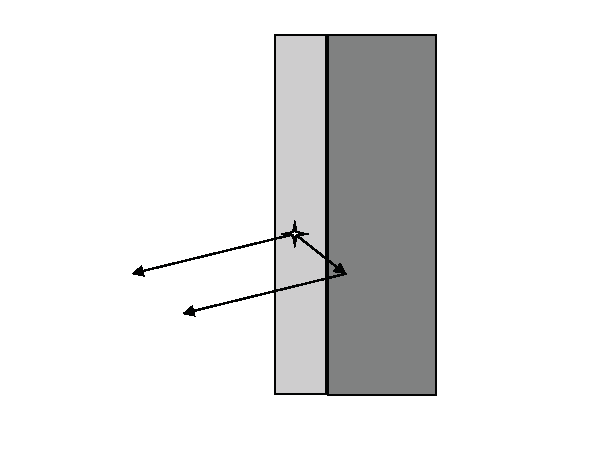
\includegraphics[scale=0.8]{DustyOpenGeometry}
\caption[Dusty open geometry]{
\label{fig:DustyOpenGeometry}The geometry assumed
in an open dusty geometry.
The lightly
shaded area is the H$^+$ region,
and is a layer on the surface of an infinitely
optically thick molecular cloud, the dark area on the right.
Light can
be emitted from the illuminated face of the cloud.
A fraction of the light
emitted towards the molecular cloud is reflected back towards the illuminated face. }
\end{figure}

\section{Continuum pumping contribution to line intensities}

Continuum pumping or fluorescence is included for all lines.
The contribution is only explicitly reported if the
\cdCommand{print line pump} command is entered.
Whether or not this contribution actually adds to the observed
line emission depends on the geometry.
Continuum pumping increases the
line emission if no related continuum absorption occurs.
This will be the
case if the continuum source is either not observed or not covered by
absorbing gas.
If absorbing gas covers an observed continuum source then
the situation is like the P Cygni problem, and pumping may not increase
the net intensity of the line at all (the absorption component will have
the same equivalent width as the associated emission).
The printed line
intensity includes this contribution unless the
\cdCommand{no induced processes} command is entered.
(The \cdCommand{no induced processes} command has many other effects and
so should only be used as a test.)

The output produced by the \cdCommand{save continuum} commands
does not include
the pumped part of the line contribution.
This is correct if the continuum
source is included in the beam, but is not if only the gas is observed.

\section{Column densities}

The column densities of all constituents are printed at the end of the
calculation.
Column densities within many excited states are also printed.
The excited states are identified with a `*'.
The table that
accompanies the description of the \cdTerm{cdColm} command
(see Table \ref{tab:cdColm_labels} on page
\pageref{tab:cdColm_labels} above)
identifies the various labels.

\section{A synthetic spectrum}

A table of emission-line intensities is part of the normal output.
Sometimes a synthetic spectrum, rather than a table, is desired.
Very coarse
spectra can be generated with the \cdCommand{save continuum} or
\cdCommand{save spectrum} commands,
but a detailed synthetic spectrum is not the main purpose of this output.

It is best to save the emission-line spectrum and then post-process this
data using your own software.  Then blends of lines can be synthesized at
any spectral resolution desired.
The spectrum can be save two ways.
The main block of emission-line intensities in the final printout
can be printed as a single column, which can be sorted by intensity
or wavelength (by using
options on the \cdCommand{print lines} command in Section 1 of this document).
The
\cdCommand{save spectrum} command includes a set of all lines with non-zero intensities.
Write a small program or script to read these tables and create a final
synthesized spectrum.

\section{Line profiles}

The observed line profile can be predicted by integrating the emissivity
of the line over the computed structure while taking the local velocity
structure into account.
The emissivity is obtained with the
\cdCommand{save lines emissivity} command,
described in Part 1 of this document.
This gives the
net emission, with units erg cm$^{-3}$~s$^{-1}$,
emitted by a unit volume of gas and
emergent from the cloud surface.
The total emission is the integral of
the emissivity.
An integral over radius will give the line intensity $4\pi J$
while an integral over volume will give the luminosity.

The observed profile will depend on the velocity field at each point
in the integration.
For static models this will be the Voigt function at
the local temperature and microturbulence.
For a dynamical model it will
include bulk motion of the gas.


     %proof 1
\include{limits}       %proof 1
\include{coninter}     %proof 2
\include{lineatomparam}%proof 1
\include{linedetl}     %proof 1
\include{CloudyStandaloneProgram} %proof 1
\include{sub}          %proof 1
\chapter{THE EMISSION LINES}
% !TEX root = hazy2.tex
\label{sec:EmissionLines}

\section{Overview}

The following sections outline the emission lines predicted by \Cloudy.
Before version 90 of the code all lines were listed in the sub-section
immediately following this section.  The code is being modified to bring
all lines into a common line class, as the code moves to C++ and objects.
This chapter will remain incomplete until this work is finished.

\section{The main emission-line printout }

The main emission line printout was briefly described
in the Chapter \cdSectionTitle{OUTPUT}.
This section
goes into more detail.

\cdCommand{Output organization}.  The printed list is sorted into four large groups
of columns, with each large column sub-divided into four smaller sub-columns.
The first sub-column is either the spectroscopic designation of the ion
producing the line or an indication of how the line is formed.  The second
sub-column is the line wavelength, with a 0 to indicate a continuum.  The
third sub-column is the log of the power in the line, in the units given
in the header (erg s$^{-1}$ into either $4\pi$ sr or cm$^{-2}$).  The last sub-column is
the intensity of the line relative to the reference line,
usually H$\beta$ , unless
this is reset with the \cdCommand{normalize} command.

These lines can be printed as a single large column, and can be sorted
by wavelength or intensity.  These options are controlled by the
\cdCommand{print line}
command described in Part I of this document.

\subsection{Intrinsic and emergent line intensities}

The computed emission-line spectrum is divided into two groups.  The
first group of lines, called ``Intrinsic line intensities'', gives the
intrinsic intensity of the lines, and does not include the reddening effects
of internal grains due to the photon's passage out of the nebula.  The second
group includes the effects of grain scattering and absorption and has the
header ``Emergent Line Intensities''.  The intensities are the total
intensities observed from the illuminated face, including both absorption
and scattering by grains.

\subsection{Line identification}

\cdCommand{Line wavelengths}.  These are given in various units.
Numbers ending
in ``A'' are wavelengths in Angstroms (\AA ).
For instance, H$\beta$ is given by ``H~~1  4861A''.
Wavelengths in microns are indicated by ``m'', an example,
the strong [O~III] IR line, is ``O~~3 51.80m''.

The code follows the convention that wavelengths longward of 2000\AA\
are given in air and shorter wavelengths in vacuum.
Continua are usually
indicated by a wavelength of zero.

\subsection{Blocks of lines\dots}

Lines are organized by common origin with a comment, ending in a series
of periods ``\dots'', beginning the section.
As an example, the first
commented block of lines begins with ``general properties\dots''.
The
following subsections give overviews of the lines.

\subsection{General properties\dots}

This mainly summarizes heating and cooling agents for the model.
\begin{description}
\item[TOTL 4861 and TOTL 1216,] are the total intensities of H$\beta$
and L$\alpha $, as
predicted by the multi-level H atom.
These intensities are the results
of calculations that include all collisional, radiative, and optical
depth effects.

\item[Inci]  The total energy in the incident continuum.
This entry will not be included if the \cdCommand{aperture} command is in effect.

\item[TotH and TotC] give the total heating and cooling.  These will be nearly
equal in equilibrium.

\item[BFH1 and BFHx] are the heating due to photoionization of ground state
and excited state hydrogen respectively.

\item[He1i, 3He1], heating due to ground state He and the triplets.

\item[BFHe and TotM] are the heating due to helium and metal photoionization.

\item[Pair] heating due to pair production.

\item[ComH , ComC],  Compton heating, cooling.

\item[CT H    CT C] charge transfer heating and cooling.

\item[extH   extC]    ``extra'' heating or cooling added to model.

\item[e-e+  511]  The positron line.

\item[Expn], expansion, or adiabatic, cooling

\item[H FB], H radiative recombination cooling

\item[HFBc, HFBc], hydrogen net free-bound cooling and heating

\item[Iind], cooling due to induced recombination of hydrogen

\item[3He2], cooling due to induced recombination of fully ionized helium

\item[Cycn], cyclotron cooling
\end{description}

\subsection{Continua\dots}

These give intensities of various continua.  These are either the total
integrated continuum or the product $\nu F_\nu$ at certain energies.

\subsubsection{Continuum bands}
The file \cdFilename{continuum\_bands.ini} in the data directory
specifies a set of wavelength bands.
The code will integrate over these bands to find the
total radiated luminosity and enter this into the main emission-line stack.
Currently this is a simple sum of the energy emitted between the upper and
lower bounds of the band, and does not take into account the transmission function
of particular instruments.
The \cdFilename{continuum\_bands.ini} file can be edited to change 
the number of bands or their detailed properties.
Table \ref{tab:continuum_bands} lists the bands in the file at the
time of this writing.
The first and second columns give
the label and wavelength as they appear in the printout.
The last column
gives the wavelength range for the integration.
These entries will not be included if the \cdCommand{aperture} command is in effect.
Please consult the file to see its current contents
and feel free to add your own bands.

%copied from ini file 2012 July 20
% commented out code to print this is in cont_createpointers.cpp
% search for string *hazy table*
\begin{table}
\centering
\caption{\label{tab:continuum_bands}Default continuum bands}
\begin{tabular}{lll}
\hline
Label& Wavelength&Wavelength Range\\
\hline
 FIR  & 83.00m & 40.00m -- 500.0m\\ 
 TIR  &  1800m & 500.0m --  3100m\\ 
 NIRa & 2.850m &  7000A -- 40.00m\\ 
 NIRb & 3.000m & 10000A -- 5.000m\\ 
 MIRa & 15.00m & 5.000m -- 25.00m\\ 
 MIRb & 22.50m & 5.000m -- 40.00m\\ 
 NMIR & 21.75m &  7000A -- 40.00m\\ 
 TFIR & 611.2m & 122.5m --  1100m\\ 
 TALL & 10000A & 0.010A -- 10000m\\ 
 F12  & 12.00m & 8.500m -- 15.00m\\ 
 F25  & 25.00m & 19.00m -- 30.00m\\ 
 F60  & 60.00m & 40.00m -- 80.00m\\ 
 F100 & 100.0m & 83.00m -- 120.0m\\ 
 MIPS & 24.00m & 20.80m -- 26.10m\\ 
 MIPS & 70.00m & 61.00m -- 80.00m\\ 
 MIPS & 160.0m & 140.0m -- 174.0m\\ 
 IRAC & 3.600m & 3.160m -- 3.920m\\ 
 IRAC & 4.500m & 4.000m -- 5.020m\\ 
 IRAC & 5.800m & 5.000m -- 6.400m\\ 
 IRAC & 8.000m & 6.500m -- 9.300m\\ 
 SPR1 & 250.0m & 212.0m -- 288.0m\\ 
 SPR2 & 350.0m & 297.0m -- 405.0m\\ 
 SPR3 & 500.0m & 414.0m -- 600.0m\\ 
 PAC1 & 70.00m & 60.00m -- 82.00m\\ 
 PAC2 & 100.0m & 84.00m -- 122.0m\\ 
 PAC3 & 160.0m & 130.0m -- 198.0m\\ 
 PAH  & 3.300m & 3.250m -- 3.350m\\ 
 PAHC & 3.230m & 3.200m -- 3.250m\\ 
 PAHC & 3.370m & 3.350m -- 3.400m\\ 
 PAH  & 6.200m & 5.900m -- 6.400m\\ 
 PAHC & 5.650m & 5.400m -- 5.900m\\ 
 PAH  & 7.900m & 7.400m -- 8.400m\\ 
 PAHC & 6.900m & 6.400m -- 7.400m\\ 
 PAH  & 11.30m & 11.10m -- 11.50m\\ 
 PAHC & 10.90m & 10.70m -- 11.10m\\ 
 PAH  & 11.80m & 11.60m -- 12.30m\\ 
 PAHC & 12.65m & 12.30m -- 13.00m\\ 
 PAH  & 13.30m & 12.90m -- 13.70m\\ 
 PAHC & 14.10m & 13.70m -- 14.50m\\ 
 Bcon &  3640A & 911.6A --  3646A\\ 
 Pcon &  5000A &  3646A --  8204A\\ 
\hline
\end{tabular}
\end{table}

\subsubsection{Other continua}

\begin{description}
\item[Bac  3646]  residual flux at head of Balmer
continuum, $\nu F_\nu$. This entry will not be included if the \cdCommand{aperture}
command is in effect.

\item[cout 3646 cref 3646], outward, reflected continuum at peak of Balmer Jump.
These entries will not be included if the \cdCommand{aperture} command is in effect.

\item[thin 3646], residual flux at head of Balmer continuum, optically thin limit.
This entry will not be included if the \cdCommand{aperture} command is in effect.

\item[Inci 4860, Inci 1215], incident continua near \ha\ and \la.
These entries will not be included if the \cdCommand{aperture} command is in effect.

\item[Ba C    0], integrated Balmer continuum

\item[PA C    0], integrated Paschen continuum

\item[HeFF    0], He brems emission

\item[HeFB    0], He recombination cooling

\item[MeFB    0], heavy element recombination cooling

\item[MeFF    0], metal brems emission

\item[ToFF    0], total brems emission

\item[FF x], part of H brems, in x-ray beyond 0.5KeV

\item[eeff], electron - electron brems
\end{description}

\cdTerm{nFnu  122m},
\cdTerm{nInu  122m},
\cdTerm{InwT  122m},
\cdTerm{InwC  122m},
a large list of continua
at selected wavelengths will be printed if the
\cdCommand{print continuum}
command is entered.
These entries will not be included if the \cdCommand{aperture} command is in effect.
The first is the sum of various continua at the wavelength,
given as $\nu F_\nu$ (see the \cdCommand{print continuum} and \cdCommand{set nFnu} commands
in Part~1 for a discussion of what is included in the \cdTerm{nFnu} entry).
\cdTerm{nInu} is the transmitted and reflected incident continuum.
\cdTerm{InwT} is the total reflected continuum.
\cdTerm{InwC} is the reflected incident
continuum.

\subsection{Molecules\dots}

\begin{description}

\item[H2dC], is the cooling due to collisional dissociation of \htwo.

\item[H2dH], heating by \htwo\ dissociation by Lyman continuum

\item[H2vH], heating by coll deexcit of vib-excited \htwo\

\item[H2vC], cooling by coll deexcit of vib-excited \htwo\

\item[H2 v], line emission by vib-excited \htwo\

\item[H-FB and H-FF] are the free-bound and free-free continua of the H- ion.

\item[H-CT 6563], H-alpha produce by H- mutual neutralization

\item[H- H]    0, H- heating

\item[H-Hc]    0, H- heating

\item[H2+] and HEH+ are the cooling due to formation of H$_2^+$ and HeH$^+$.

\item[Codh], carbon monoxide photodissociation heating

\item[CO C   12], C12O16 cooling

\item[CO C   13], C13O16 cooling

\end{description}

\subsection{Grains\dots}

Information in this block concerns emission, absorption, heating, and
cooling by any grains included in the calculation.

\begin{description}
\item[GrGH], gas heating by grain photoionization

\item[GrTH], gas heating by thermionic emissions of grains

\item[GrGC], gas cooling by collisions with grains

\item[GraT], This is the total grain heating by all sources, lines, collisions,
incident continuum.  If the grain emission is optically thin limit then
this is equal to the total intensity in grain emission.

\item[GraI], grain heating by incident continuum

\item[GraL 1216], grain heating due to destruction of L$\alpha $

\item[GraC], grain heating due to collisions with gas

\item[GraD], grain heating due to diffuse fields, may also have grain emission
\end{description}

Grain emission is included in the predicted total emitted continuum.
A machine readable form of the continuum can be produced with the \cdCommand{save continuum} command,
also described in Part I of this document.

\subsection{H-like iso-seq\ldots}

This block includes all hydrogen-like isoelectronic species.
The \cdCommand{atom H-like} command,
described in Part 1 of this document, adjusts properties
of this sequence.

\begin{description}
\item[HFFc    0], net free-free cooling, nearly cancels with cooling in lte

\item[HFFh   0], net free-free heating, nearly cancels with cooling in lte

\item[H FF   0], H brems (free-free) cooling

\item[FF H    0], total free-free heating

\item[Clin  912], total collisional cooling due to all hydrogen lines

\item[Hlin  912], total collisional heating due to all hydrogen lines

\item[Cool 1216], collisionally excited La cooling

\item[Heat 1216], collisionally de-excited La heating

\item[Crst  960], cooling due to n>2 Lyman lines

\item[Hrst  960], heating due to n>2 Lyman lines

\item[Crst 4861], cooling due to n>3 Balmer lines

\item[Hrst 4861], heating due to n>3 Balmer lines

\item[Crst    0], cooling due to higher Paschen lines

\item[Hrst    0], heating due to higher Paschen lines

\item[LA X 1216], L$\alpha $ contribution from suprathermal secondaries from ground

\item[Ind2 1216], L$\alpha $ produced by induced two photon

\item[Pump 4861], H$\beta$ produced by continuum pumping in optically thin ld limit

\item[CION    0], net col ionz-3 body heat collision ionization cooling of
hydrogen

\item[3bHt    0], heating due to 3-body recombination

\item[Strk 1216], Stark broadening component of line

\item[Dest 1216], part of line destroyed by background opacities

\item[Fe 2 1216], part of L$\alpha $ absorbed by Fe II

\item[Q(H) 4861] is the intensity of H$\beta$ predicted from the total number of
ionizing photons, Q(H$^0$), assuming that each hydrogen-ionizing photon produces
one hydrogen atom recombination. This entry will not be included if the \cdCommand{aperture}
command is in effect.

\item[Q(H) 1216] indicates the L$\alpha $ intensity produced if each hydrogen ionizing
photon results in one \la\  photon in the high density limit (i.e., no
two-photon emission). This entry will not be included if the \cdCommand{aperture}
command is in effect.

\item[CaBo 4861] These are the ``old'' case B predictions, as printed in versions
90 and before of the code.
\end{description}

\cdTerm{Ca B 6563A} The entries starting with ``Ca~~B''
are the Case B intensities
computed from the actual model ionization and temperature structure, but
assuming that H$\beta$ emits with its Case~B emissivity.

Next the predicted intensities of all lines of the hydrogenic
iso-electronic sequence are given.
The lines have labels that identify
the species and stage of ionization,
such as ``H~~1'', ``He~2'', ``Li~3'', ``C~~6'', etc.
The entries with a wavelength of zero are the total intensities
of the $2s-1s$ two-photon emission.

\subsection{He iso-sequence\dots }

Atoms and ions of the helium-like iso-electronic sequence are treated
as multi-level atoms.  All species and stages of ionization are specified
by labels like ``He~1'', ``Li~2'', ``C~~5'', etc.
A wavelength of zero indicates the
two-photon continuum.
The $2\;^3P$ term is resolved into three levels.
Emission of
each line of the $2\;^3S - 2\;^3P$ and $1\;^1S - 2\;^3P$ multiplets
is predicted along with the sum of
the multiplets with label ``TOTL''.
The \cdCommand{atom He-like} command, described in Part 1 of
this document, adjusts properties of this sequence.
Further details are
given in \citet{Bauman2005}, \citet{Porter2005}, and \citet{PorterFerland2007}.

\subsection{level 1 lines\ldots}

In the current version of the code, the lines printed under this title
include both the lines that have been moved to the
\cdVariable{EmLine} class,
but also older lines that are still scalar quantities.
This part of the
code is still in a state of flux, and this is reflected in the current
documentation.
The remaining part of this subsection outlines the methods
used for most of the heavy element atoms.
The method for producing a list
of transferred lines,
those that have been moved to the \cdFilename{EmLine} class, is
described in the section beginning on
page \pageref{sec:TransferredLines} below.

These lines have accurate collision strengths and wavelengths.
Many
are two-level atoms, but some are the result of multi-level atoms.
The
following is a summary of the general approach.

\cdCommand{Li-sequence}.  Examples include C~IV $\lambda $1549,
O~VI $\lambda $1034, and Mg~II $\lambda $2798.
A three-level atom, with full treatment of optical depths and collisional
excitation, is used.  The ``TOTL'' intensity is the sum of both lines in
the doublet, and is followed by the individual intensities of each member.

\cdCommand{Be-sequence}.  Examples include C~III] $\lambda$ 1909,
O~V] $\lambda $1215, and Si~III] 1895.
A four-level atom, solving for populations of the
individual $^3P_j$ states, is used.
The first printed intensity is the total intensity of the multiplet
(both $j=0$,1 decays) and this is followed by the intensities of
individual lines.
The intensity of the permitted $^1P_o - ^1S$ transition is also
calculated.  Optical depth and collisional effects on both the permitted
and intercombination lines are included.

\cdCommand{B-sequence}.  Examples include C~II and O~IV.
The ground term is treated
as a two level atom, with optical depth and collisional effects included,
when the gas is too cool to excite the UV lines.
The $^4P -^2P_o$ lines are
also predicted with a full multi-level atom that resolves fine structure.
The ``TOTL'' intensity printed is the total intensity
of the multiplet and is
followed by individual lines.
Pumping by all level-two lines of the same
ion is included as an excitation process.

\cdCommand{$^3$P- ground term}. Examples include such spectra as [O~III] and [O~I].
The infrared fine structure lines are computed with full treatment of
collisional and optical depth effects.
A comment is printed at the end
of the model if these lines mase or become optically thick.
The populations
of $^1D$ and $^1S$ are computed with a three-level atom.
The intensity of the
$^1D - ^3P$ transition is only that of the individual line
(i.e. 5007), not the doublet.

\cdCommand{$^4$S$^0$ - ground term}.  Examples include [O~II] and [S~II].  They are treated as a five-level atom.
Intensities of all individual lines, as well as
co-added multiplets, are given.

\subsection{Recombination\dots}

These are a set of heavy-element recombination lines that are predicted
in the low-density limit assuming that the transitions are optically thin.
This consists of all recombination lines of C, N., and O, with coefficients
taken from \citet{Nussbaumer1984} and \citet{Pequignot1991}.

These predictions are for optically thin pure recombination.
These should
be accurate for planetary nebulae and H II regions.
They will not be
accurate for dense environments where optical depths and collisional effects
come into play.
These are only included in the output if the electron
density is less than $10^8 \pcc$,
a rough upper limit to the range of validity
in the original calculations of the coefficients.

There are several instances where more than one line of an ion will have
the same wavelength due to the integer Angstrom format used for wavelengths.
The worst case is O~V 4953,
where three lines of the same multiplet have
the same wavelength.

\subsection{Level 2 lines\dots }

These are resonance lines that use Opacity Project wavelengths, which
are generally accurate to about 10\%.
These lines have g-bar collision
strengths, which are not very accurate at all.

\section{The transferred lines}
\label{sec:TransferredLines}

\subsection{Save line data output}

The group of ``transferred lines'' includes all those that have been
moved to the \cdFilename{EmLine} class.

In older versions of this document a large list of emission lines
appeared here.
This list is now far too large to include here.
Rather,
the list can be generated by executing the code with the command \cdCommand{save line data ``filename.txt''} included.
This will create a file that includes the
full set of lines that are predicted.
Note that the lines that are output
are only those that exist when the code is run.
It is possible to make
many of the model atoms and molecules as large or small as you like,
and
the actual lines that exist when the \cdCommand{save} command
is entered will be output.
The test case \cdFilename{func\_lines.in} in the test suite
includes this save command and generates a list of all transferred
lines in the file \cdFilename{func\_lines.lis}.

To generate a line list, set up a calculation with the atoms set to
whatever size is desired (see the \cdCommand{atom} command in Part I).  Then execute
this script with the \cdCommand{save line data} command included (described in Part I).
The save output will include the line list.
This will include the
level 1 ,level 2, \htwo, \feii, CO, and recombination lines,
but not the scalar forbidden lines.
These are described in a list following this subsection.

This contains several groups of lines.
All quantities were evaluated at $10^4 \K$.
The description of the command in Part I of this document explains
how to evaluate the quantities at other temperatures.

The ion is the first column of the table.
This is in a uniform format,
beginning with the two character element symbol and followed by an integer
indicating the level of ionization.
``C~~2'' is C$^+$ or C~II.
This is
followed by the integer wavelength label used to identify the line in the
printout.
The third column, with the label ``WL'', is the correct wavelength
of the line, with units of microns (``m''), Angstroms (``A''),
or cm (``c'').
The remaining columns give the statistical weights of the lower and upper
levels, the product of the statistical weight and the oscillator strength,
and then the transition probability.

The last column is the electron collision strength.
Usually these collision strengths
are for only the indicated transition, although in some cases (the Be
sequence) the value is for the entire multiplet.

\subsection{Output produced for the transferred lines}

Because the lines have a common format within their storage vectors,
the output has a common format too.
Generally only the total intensity
of the transition, the result of the solution of a multi-level atom with
all processes included, is printed.
The approach used to compute the level
populations is described in Part II of \Hazy,
and includes continuum pumping,
destruction by background opacities, and trapping.

The total intensity of the transition is printed in a form like ``C~~2 1335'', with the spectroscopic identification given by the first part,
as found in the first column of the table, and the wavelength as indicated
by the number in the second column of the table.

In a few cases (for instance, the C~IV $\lambda \lambda $1548, 1551 doublet), a total
intensity is also derived.
In these cases the label ``TOTL'' will appear
together with an average wavelength (1549 in this case).
These lines are
all explicitly shown in a following section.

It is possible to break out various contributors to the lines with options
on the \cdCommand{print line} command, described in Part I of this document and in the
following.
These contributors are printed following the total intensity.

\cdCommand{print line heating}  An emission line will heat
rather than cool the gas
if it is radiatively excited but collisionally de-excited.
The print out
will include this agent, with the label ``Heat'',
when this command is given.

\cdCommand{print line collisions}  The collisional contribution
to the lines will
be printed, with the label ``Coll''.

\cdCommand{print line pump}  The contribution to the total line, produced by continuum
pumping, is printed with the label ``Pump''.   What is observed?  Whether
or not this is a net emission process contributing to the observed line
intensity depends on the geometry, mainly whether or not continuum source
is in the beam. At some velocities within the line profile this can be a
net emission process, due to absorption at other velocities.   If the
continuum source is in the beam and gas covers it, this is not a net emission
process, since photons are conserved.

\cdCommand{print line inward}  The inwardly directed part of the total emission is
printed with the label ``Inwd''.  This can be greater than half of the line
intensity if the line is optically thick since these lines tend to be
radiated from the hotter illuminated face of the cloud.

\cdCommand{print line optical depths}  At the end of the calculation the optical
depths for all optically thick lines will be printed.
This is not done
by default since it can be quite long.

\section{Line identifications}

The file \cdFilename{line\_labels.txt} in the docs directory of the distribution lists
line identifications and a brief description of its origin.

\section{Hydrogen recombination lines}

Table \ref{tab:HydrogenEmissionLines} gives the strongest lines
of the lowest series.
All lines have the label ``H~~1''.
The wavelength column gives
the string as it appears in the printout.  ``m'' indicates a wavelength
in $\mu$m and A in Angstroms.
The Case B intensity is taken from the
\cdFilename{limit\_caseb\_h\_hs87} test case.

Some IR lines may have the same wavelength if the default line precision is used.
The \cdCommand{set line precision} command can be used 
to increase the number of significant figures in the
line wavelength, which should make identification easier.

\begin{table}
\centering
\caption{\label{tab:HydrogenEmissionLines}Hydrogen emission lines}
\begin{tabular}{llll}
\hline
Series& $n'\to n$& Wavelength& $I$(Case B)\\
\hline
Lyman& 2--1& 1216A& - \\
Balmer H$\alpha$& 3--2& 6563A     &2.8463\\
H$\beta$& 4--2& 4861A     &1.0000\\
H$\gamma$& 5--2& 4340A     &0.4692\\
H$\delta$& 6--2& 4102A     &0.2596\\
Paschen P$\alpha$& 4--3& 1.875m   & 0.3319\\
P$\beta$& 5--3& 1.282m    &0.1617\\
P$\gamma$& 6--3& 1.094m    &0.0899\\
P$\delta$& 7--3& 1.005m    &0.0553\\
Brackett Br$\alpha$& 5--4& 4.051m &    0.0778\\
Br$\beta$& 6--4& 2.625m&     0.0445\\
Br$\gamma$& 6--4& 2.166m&     0.0274\\
Br$\delta$& 6--4& 1.945m&     0.0180\\
Pfund& 6--5& 7.458m& 0.0246\\
Humphreys& 7--6& 12.37m& 0.0098\\
& 8--7& 19.06m& 0.0042\\
& 9--8& 27.80m& 0.0020\\
\hline
\end{tabular}
\end{table}

\section{Molecular hydrogen lines}

Table \ref{tab:MolecularHydrogenLines} gives some of the stronger
or more frequently observed \htwo\ lines.
These are only predicted when the large model \htwo\ molecule is
included with the \cdCommand{atom H2} command.
The wavelength column gives the string
as it appears in the printout.  ``m'' indicated a wavelength in $\mu$m.
All lines have the label ``H2~~''.

Many lines will have the same wavelength if the default line precision is used.
The \cdCommand{set line precision} command can be used 
to increase the number of significant figures in the
line wavelength, which should make identification easier.

\begin{table}
\centering
\caption{\label{tab:MolecularHydrogenLines}Molecular hydrogen emission lines}
\begin{tabular}{lllll}
\hline
Transition& $v_{hi},J_{hi}$& $v_{lo},J_{lo}$& $\lambda$(label)& $\chi$(hi,
K)\\
\hline
0-0 S(0)& 0,2& 0,0& 28.21m& 509.8\\
0-0 S(1)& 0,3& 0,1& 17.03m& 1015.1\\
0-0 S(2)& 0,4& 0,2& 12.28m& 1681.6\\
0-0 S(3)& 0,5& 0,3& 9.662m& 2503.8\\
0-0 S(4)& 0,6& 0,4& 8.024m& 3474.3\\
0-0 S(5)& 0,7& 0,5& 6.907m& 4586.2\\
0-0 S(6)& 0,8& 0,6& 6.107m& 5829.5\\
1-0 O(2)& 1,0& 0,2& 2.626m& 5986.9\\
1-0 Q(1)& 1,1& 0,1& 2.406m& 6149.0\\
1-0 O(3)& 1,1& 0,3& 2.802m& 6149.0\\
1-0 S(0)& 1,2& 0,0& 2.223m& 6471.4\\
1-0 Q(2)& 1,2& 0,2& 2.413m& 6471.4\\
1-0 O(4)& 1,2& 0,4& 3.003m& 6471.4\\
1-0 S(1)& 1,3& 0,1& 2.121m& 6951.3\\
1-0 Q(3)& 1,3& 0,3& 2.423m& 6951.3\\
1-0 O(5)& 1,3& 0,5& 3.234m& 6951.3\\
0-0 S(7)& 0,9& 0,7& 5.510m& 7196.7\\
1-0 S(2)& 1,4& 0,2& 2.033m& 7584.3\\
1-0 Q(4)& 1,4& 0,4& 2.437m& 7584.3\\
1-0 O(6)& 1,4& 0,6& 3.500m& 7584.3\\
1-0 S(3)& 1,5& 0,3& 1.957m& 8365.0\\
1-0 Q(5)& 1,5& 0,5& 2.454m& 8365.0\\
1-0 O(7)& 1,5& 0,7& 3.806m& 8365.0\\
0-0 S(8)& 0,10& 0,8& 5.051m& 8677.0\\
1-0 S(4)& 1,6& 0,4& 1.891m& 9286.3\\
1-0 Q(6)& 1,6& 0,6& 2.475m& 9286.3\\
0-0 S(9)& 0,11& 0,9& 4.693m& 10261\\
1-0 S(5)& 1,7& 0,5& 1.835m& 10341\\
1-0 S(6)& 1,8& 0,6& 1.787m& 11521\\
1-0 S(7)& 1,9& 0,7& 1. 748m& 12817\\
\hline
\end{tabular}
\end{table}

The following is an example which predicts the emissivity of the \htwo\ 2.121 1-0 S(1) \micron\ line.
\begin{verbatim}
save line emissivity ``lines.ems''
H2   2.121m
end of lines
\end{verbatim}

A list of all H2 lines with their labels and excitation energies can
be generated with the command \cdCommand{save H2 lines}.
\href{http://jach.hawaii.edu/UKIRT/astronomy/calib/spec\_cal/h2\_s.html}{The Joint Astronomy Centre} in Hawaii give a
summary of \htwo\ lines.

\section{CO lines}

Rotation transitions within the ground vibration level are included.  
These are listed in Table \ref{tab:COLines} which gives the symbol
``m'' to indicate $\micron$.

\begin{table}
\centering
\caption{\label{tab:COLines}CO emission lines}
\begin{tabular}{ll}
\hline
Label & wavelength \\
\hline
CO   & 2600m \\
CO   & 1300m \\
CO   & 866.7m \\
CO  	& 650.1m \\
CO  	& 520.1m \\
CO  	& 433.4m \\
CO  	& 371.5m \\
CO  	& 325.1m \\
CO  	& 289.0m \\
CO  	& 260.2m \\
CO  	& 236.5m \\
CO  	& 216.9m \\
CO  	& 200.2m \\
CO  	& 185.9m \\
CO  	& 173.6m \\
CO  	& 162.8m \\
CO  	& 153.2m \\
CO  	& 144.7m \\
CO  	& 137.2m \\
CO  	& 130.3m \\
CO  	& 124.2m \\
CO  	& 118.5m \\
CO  	& 113.4m \\
CO  	& 108.7m \\
CO  	& 104.4m \\
CO  	& 100.4m \\
CO  	& 96.75m \\
CO  	& 93.32m \\
CO  	& 90.14m \\
CO  	& 87.17m \\
CO  	& 84.39m \\
CO  	& 81.78m \\
CO  	& 79.34m \\
CO  	& 77.04m \\
CO  	& 74.87m \\
CO  	& 72.82m \\
CO  	& 70.89m \\
CO  	& 69.06m \\
CO  	& 67.32m \\
CO  	& 65.67m \\
\hline
\end{tabular}
\end{table}

        %proof 1
\include{problems}     %proof 1
\include{odetail}      %proof 1
\appendix
\include{sources}      %proof 1
\include{glossary}     %proof 1
\include{conversion}   %proof 1
\include{TestSuite}
\backmatter
\bibliographystyle{plainnat}
\bibliography{../common/bibliography2}

\end{document}
